In esso la dislocazione delle cariche è totale, per cui immaginiamo che ci sia cessione dell'elettrone e in conseguenza a ciò si formino uno ione positivo e uno negativo.

\subsection{Considerazioni energetiche nella formazione di un legame ionico}
Immaginiamo di avere due atomi separati, ad esempio litio e fluoro.

Nella specie LiF effettivamente si hanno ioni litio e fluoruro, ossia il litio ha ceduto il suo unico elettrone esterno al fluoro.

Se il litio cede un elettrone, vuol dire che è stata spesa dell'energia per strapparglielo, per esattezza si deve spendere una energia pari a quella di prima ionizzazione del litio, che ammonta a 520 kJ/mol.
Al contempo, poiché il fluoro sta acquistando un elettrone, dovrà emettere una certa quantità di energia pari alla sua affinità elettronica, che vale -328 kJ/mol. Questo significa che essa da sola non basta a ionizzare il litio, ossia se mettessimo vicini ma isolati due atomi, uno di fluoro e uno di litio, non si formerebbero questi ioni, in quanto il fluoro tenderebbe a catturare l'elettrone del litio, ma libererebbe un'energia non sufficiente a ionizzare il litio, poiché tale processo richiede più energia.

Ne segue che questi due atomi isolati non daranno luogo alla specie molecolare Li$^+$F$^-$.

Considerazioni analoghe valgono per qualsiasi altro composto ionico, come ad esempio l'NaCl: l'affinità elettronica del cloro non è sufficiente a strappare l'elettrone al sodio affinché diventi Na$^+$, in quanto il suo potenziale di prima ionizzazione è più alto dell'affinità elettronica del cloro, per cui la molecola NaCl non può esistere come singola entità.

Tuttavia sia il fluoruro di litio, che il cloruro di sodio, esistono.

Dobbiamo quindi trovare la fonte di questo legame, cioè capire perché esiste il solido ma non la molecola singola.

La prima domanda che quindi ci poniamo è: "Dove sta la forza che tiene legati insieme questi ioni, dato che il sistema solido esiste?"

Una prima risposta è che essa deve stare nella struttura adottata in fase solida. È lì che dobbiamo cercare la ragione, perché se la molecola non esiste e il solido si è chiaro che in quest'ultimo ci sarà un qualche contributo in energia che permette la formazione della specie chimica.

Per mostrare la validità di tale ipotesi utilizziamo un ciclo termodinamico chiamato \textbf{Ciclo di Born-Haber}, che permette di razionalizzare la ragione dell'esistenza dei solidi di tutti i sistemi ionici.

Il nostro obiettivo è capire perché possiamo prendere del litio solido Li$_{(s)}$, aggiungere del fluoro gassoso F$_{(g)}$ e ottenere il fluoruro di litio solido LiF$_{(s)}$ senza problemi.

Il fluoruro di litio presenta una struttura solida nella quale ioni litio e ioni fluoruro occupano precise posizioni reticolari, quindi non è una struttura disordinata, anzi è estremamente ordinata.

L'energia che stiamo cercando è la variazione di entalpia che si ha nella formazione del solido ionico a seguito della reazione:
$$\ce{Li^{+}_{(g)} + F^{-}_{(g)} -> LiF_{(s)}} \quad \Delta\text{H=?}$$
In questa reazione una mole di litio gassoso reagisce con una mole di fluoro gassoso per dare luogo ad una mole di fluoruro di litio solido, in quanto non esiste in forma gassosa.

Purtroppo questa reazione è impossibile da realizzare, perché in natura non abbiamo né ioni litio gassosi, in quanto il litio è presente solo come composto insieme a qualche altro elemento, né ioni fluoruro gassosi, in quanto esiste in forma molecolare F$_2$. Pertanto non possiamo partire da questi reagenti.

Quello che possiamo fare è partire dai composti del litio, fonderli, fare elettrolisi e ridurre il Li$^+$ a Li$^0$ tramite processi elettrochimici. Dopodiché facciamo reagire questo insieme al fluoro gassoso e otteniamo:
$$\ce{Li_{(s)} + \frac{1}{2}F_{2(\text{g})} -> LiF_{(s)}}$$
Notiamo che questa reazione è diversa da quella di partenza, ma se stiamo attenti a lavorare a pressione costante, le energie scambiate diventano variazioni di entalpia $\Delta$H, che è una funzione di stato, per cui non dipenderà dal particolare percorso, ma solo da stato iniziale e finale. In altre parole possiamo fare avvenire questa reazione tramite il percorso diretto o tramite il percorso più complesso, contenuto all'interno del ciclo di Born-Haber, e la variazione di energia che si ha passando da reagenti a prodotti sarà la stessa. Ciò è possibile grazie alla \textbf{Legge di Hess}, la quale afferma che:

\vspace{0.2cm}"\textit{Il calore scambiato a pressione costante in una reazione chimica che possa essere scomposta in più reazioni parziali è indipendente dagli stati intermedi attraverso i quali si evolve il sistema e dipende solo dagli stati iniziale e finale. La variazione di calore è pari alla somma algebrica delle variazioni di calore dei singoli stadi.}"

\vspace{0.2cm}A causa di tale legge, se abbiamo calori scambiati a pressione costante il sistema può essere rappresentato attraverso una serie di stati intermedi, ottenendo così un ciclo termodinamico e quindi le energie coinvolte dipendono solo dallo stato iniziale e da quello finale.

\vspace{0.2cm}Il processo che si usa è il seguente:
\begin{itemize}
    \item Si parte dal litio solido e si spende una certa energia $\Delta\text{H}_{atomiz}$ per portarlo in fase gassosa che chiamiamo energia di atomizzazione o evaporazione del litio, facilmente misurabile con un calorimetro.
    \item Si rompe la molecola biatomica del fluoro, passando così da F$_2$ a 2F. L'energia così spesa è quella di dissociazione del fluoro che è detta \textit{binding energy} $(BE)$. Poiché ci serve solo un atomo di fluoro e da ogni molecola ne otteniamo due, ci basta metà di questa energia.
    
    A questo punto avremo litio e fluoro entrambi allo stato gassoso.
    \item Si fornisce l'energia di prima ionizzazione $IP_1$ del litio per ottenere il suo catione: $\ce{Li_{(g)} -> Li^{+}_{(g)} + 1e}$
    \item L'elettrone ottenuto dalla ionizzazione del litio viene acquistato dal fluoro, il quale diventa F$^-$ e cede un'energia pari alla sua affinità elettronica $EA$.
    \item Arriviamo così ad avere ioni Li$^+$ e F$^-$ gassosi, che sono i reagenti della reazione considerata inizialmente, la quale ci interessa poiché in essa vi è tutta la stabilità del sistema solido.
    
    Essi insieme daranno luogo al fluoruro di litio solido e quindi pur non avendo fatto il percorso diretto siamo arrivati allo stesso prodotto.
\end{itemize}

\vspace{-0.4cm}\begin{figure}[H]
    \centering
    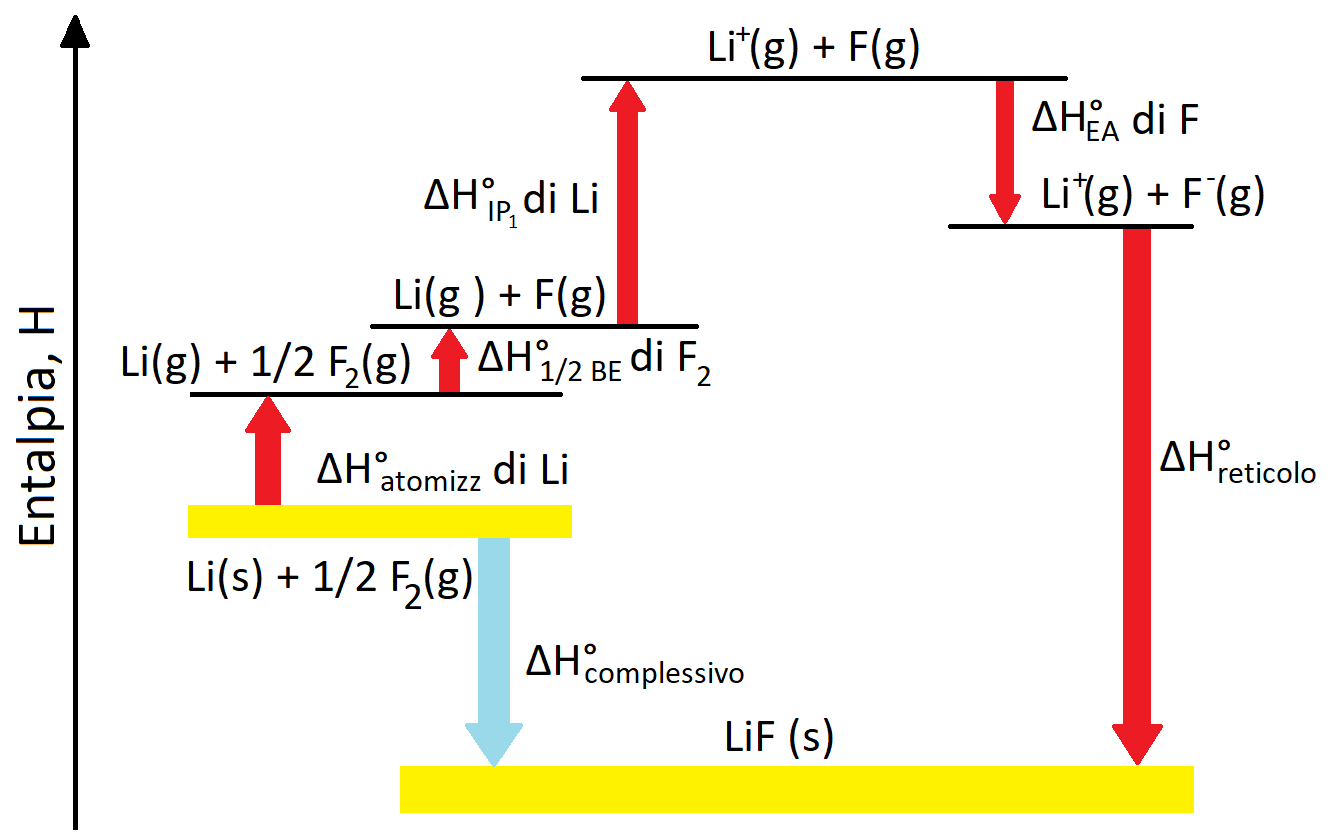
\includegraphics[width=12cm]{immagini/Ciclo-Born-Haber.png}
\end{figure}

\vspace{-0.2cm}Poiché stato iniziale e stato finale sono gli stessi, la somma di tutti questi calori deve essere uguale al calore scambiato nel percorso diretto.

Il calore di formazione emesso nel processo diretto lo sappiamo calcolare, mentre nel processo complesso non sappiamo misurare solo il calore emesso per passare dagli ioni gassosi al reticolo solido, il quale però può essere calcolato facendo la differenza tra valori sperimentali:
$$\Delta\rm{H}_{reticolo}=\Delta\rm{H}_{complessivo} - \Delta\rm{H}_{atomiz} - \Delta\rm{H}_{BE} - \Delta\rm{H}_{IP_1} + \Delta\rm{H}_{EA}$$
Si trova che, alla temperatura di 25° C e alla pressione di 1 bar, il $\Delta$H complessivo è pari a -617 kJ/mol. È negativo perché quando mettiamo insieme litio e fluoro spontaneamente si forma il fluoruro di litio, emettendo tale calore.

Facendo la differenza tra tale calore e gli altri calori misurabili si trova che l'energia di reticolo vale -1050 kJ/mol, che viene emessa con la formazione del reticolo.

Quindi il legame chimico nei sistemi ionici sta tutto nella formazione del reticolo, cioè la stabilità del solido e la inesistenza della singola molecola sta nel fatto che in questa l'energia emessa dal fluoro quando acquista un elettrone non basta a ionizzare il litio, che è quello che dovrebbe cedere l'elettrone, per cui la molecola non potrà formarsi, mentre quando si forma il solido questi ioni liberano una grande quantità di energia, cosa che permette al solido di formarsi. Quindi è proprio all'interno del reticolo che si trova la stabilità di questo sistema: quando questi ioni vanno ad occupare precise posizioni reticolari si forma questo reticolo estremamente stabile con l'emissione di una quantità molto grande di energia.

Questo discorso vale per tutti i solidi ionici: non esistendo le loro molecole ma il loro solido si, vuol dire che la stabilità è conferita dall'arrangiamento in fase solida.

\vspace{0.2cm}N.B.: Se chiede di parlare del legame ionico attraverso un modello termodinamico descrivi il ciclo, ma se chiede perché abbiamo la necessità di usare il ciclo, il motivo è perché siamo interessati al $\Delta\rm{H}_{reticolo}$, che è l'energia del reticolo cristallino, perché in tale reazione da un lato abbiamo gli ioni gassosi e dall'altro abbiamo il solido con un reticolo cristallino, per cui vogliamo conoscere l'energia che viene emessa quando quest'ultimo si forma, ossia partiamo da un'energia molto alta di questi ioni $\rm Li^+$ e $\rm F^-$ gassosi e quando questi si uniscono per formare il solido emettono una quantità enorme di energia, e il sistema si stabilizza tantissimo. Questa energia emessa si chiama \textit{energia reticolare} perché è l'energia del reticolo. Quindi in questo secondo caso la prima cosa da dire è: "L'energia reticolare è l'energia associata al processo nel quale sono reagenti, in questo caso particolare, ione litio gassoso più ione fluoruro gassoso, e il prodotto è il fluoruro di litio, ma noi non siamo in grado di effettuare questa reazione, perché questi reagenti non li abbiamo. Ecco perché usiamo il ciclo di Born-Haber, il quale ci permette di aggirare questo problema". Dopodiché si inizia a parlare del ciclo, quindi diamo la motivazione (voler conoscere l'energia del reticolo, che è quella che tiene insieme gli ioni nel reticolo).

\subsection{Differenze tra composti molecolari e composti ionici}
Per i composti molecolari esistono le singole molecole, per quelli ionici no: essi esistono solo in forma di reticolo cristallino, dove gli ioni occupano posizioni ben precise, alternandosi, in tutte e tre le direzioni. Ne segue che per questi si parla di \textbf{unità formula}.

La conseguenza di ciò è che se mettiamo in acqua ad esempio il glucosio $\rm C_6H_{12}O_6$, che è un composto molecolare, esso resta tale, mentre se mettiamo ad esempio il cloruro di sodio NaCl esso si dissocia in ioni Na$^+$ e Cl$^-$. Ciò che avviene è che l'acqua aggredisce il cristallo e stacca singoli ioni, i quali vengono portati in soluzione con delle molecole di acqua che li circondano. In particolare gli ioni positivi saranno circondati dagli atomi di ossigeno dell'acqua, in quanto essi reagiranno con la parziale carica negativa presente su questo, mentre gli ioni negativi saranno circondati dagli idrogeni dell'acqua poiché interagiranno con la parziale carica positiva presente su questi:

\vspace{-0.3cm}\begin{figure}[htp]
    \centering
    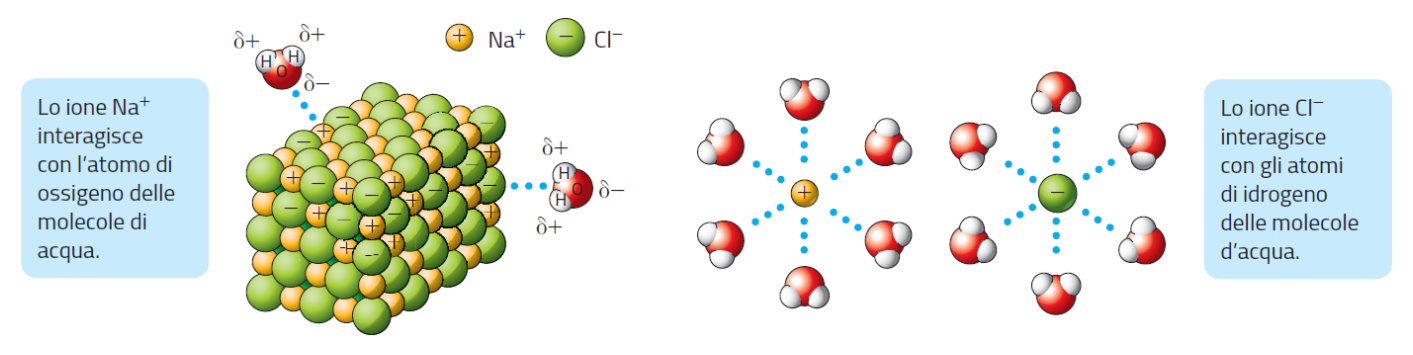
\includegraphics[width=15cm]{immagini/interazione-acqua-ioni.png}
\end{figure}

\vspace{-0.3cm}Dunque in soluzione si avranno ioni.

L'evidenza sperimentale di tale fatto si ottiene confrontando tre circuiti elettrici con una lampadina, dove in uno inseriamo in serie dell'NaCl solido, in un altro dell'NaCl fuso e in un terzo una soluzione di NaCl sciolto in acqua. Il primo non permette la conduzione (la lampada non si accende), il secondo permette una leggera conduzione (la lampada si accende ma la luce è fioca), il terzo permette una grande conduzione (la lampada si accende con luminosità maggiore).

\begin{figure}[htp]
    \centering
    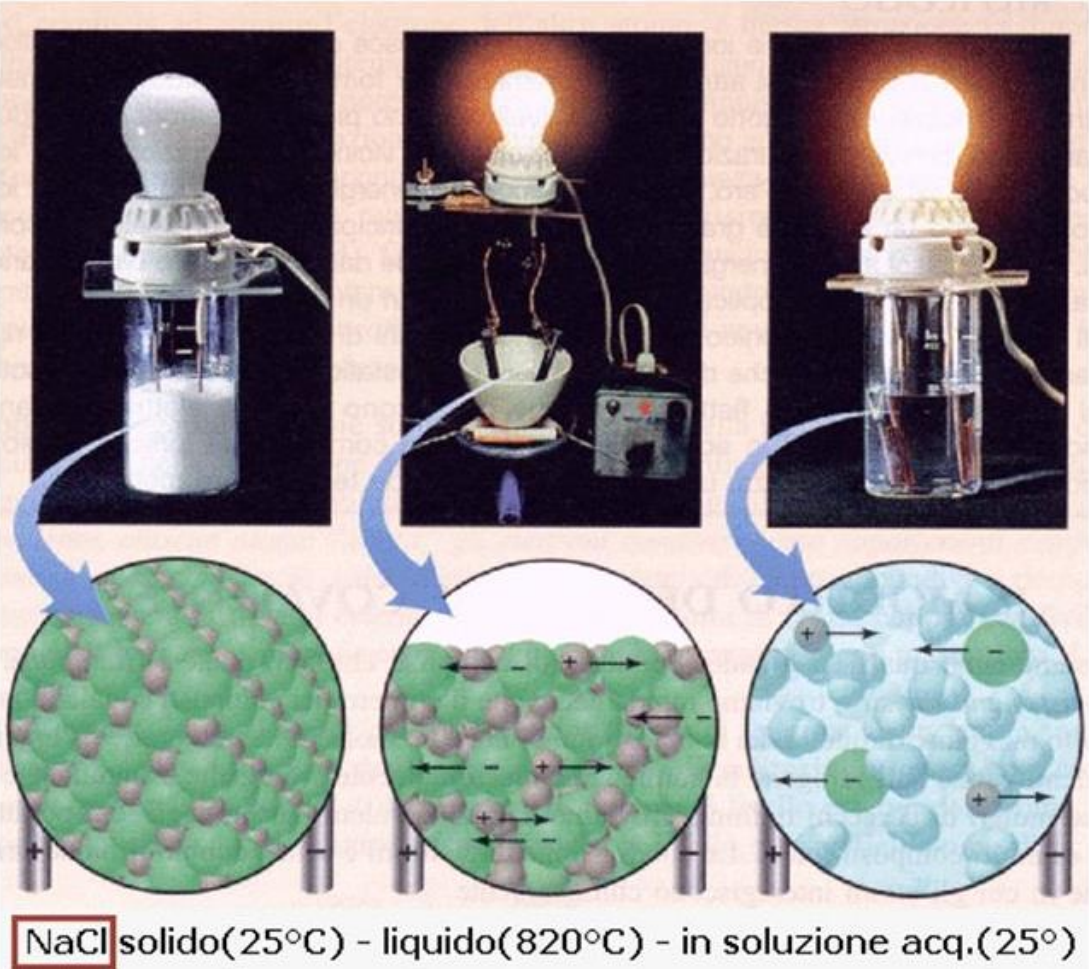
\includegraphics[width=9cm]{immagini/lampadina.png}
\end{figure}

Tale esperimento mostra l'esistenza degli ioni, che sono i portatori di carica che permettono la conduzione.

Se invece avessimo collegato a lampadina ad una soluzione acquosa contenente zucchero, la lampadina non si accenderebbe. Il motivo è che lo zucchero è un composto molecolare, per cui non si scioglie in acqua e non dà origine a ioni.
\subsection{Proprietà fisiche dei composti ionici}
Tipicamente i composti ionici sono duri, rigidi e fragili, cioè è facile romperli.

Se solidi, non conducono elettricità, per cui costituiscono dei buoni isolanti. Se invece li portiamo a fusione (che per tali composti significa portarli ad una temperatura di 800-1000°C) iniziano a condurre. Se invece li sciogliamo in acqua la mobilità degli ioni diventa elevata e la conducibilità è ancora maggiore. Tale fatto è la dimostrazione dell'esistenza degli ioni come portatori di carica.

In genere hanno temperature di fusione elevate, perché dobbiamo abbattere l'energia reticolare, che è molto elevata, per poter liberare gli ioni dal reticolo.

All'interno dei reticoli gli ioni sono disposti alternatamente nelle varie direzioni
\begin{figure}[htp]
    \centering
    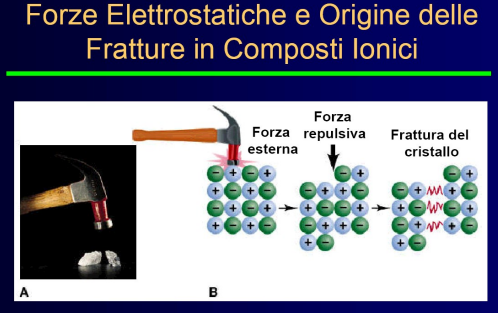
\includegraphics[width=9cm]{immagini/struttura-composti-ionici.png}
\end{figure}

Immaginiamo un sistema bidimensionale. Se cerchiamo di rompere il cristallo, lo si deve spezzare e far scivolare il sistema in un piano. Se riusciamo a fare ciò, riusciamo a rompere il cristallo.